%************************************************
\chapter{Discussion}\label{ch:discussion}
%************************************************


\section{Summary}

\section{Limitations}

Need for explicit modeling of learning process.

Need for operational definitions based on mechanistic process theories

\subsection{Perception}

    Arousal of curiosity is due to encounters with stimulus-events characterized as novel, complex, or ambiguous. These characteristics imply that information about said stimulus-events is missing. Thus, curiosity is aroused when the observer detects deficiencies in its knowledge. While terms like "novel", "complex", and "ambiguous" are typically used to describe stimuli, it would be more accurate to say that they describe particular states of the observer's representations activated by the stimuli. Thus, novelty, complexity, and ambiguity are products of subjective perception, not objective features of the stimuli.

    Consider one of the current accounts of visual perception. The process by which objects are perceived as such can be understood as a sequence of inferences of progressively higher-level representational encodings simultaneously informed by bottom-up activity (the data) and constrained by top-down activity (prior knowledge; Bruno Olshausen, 2013, In The Cognitive Neurosciences, Gazzaniga & Mangun (Eds)). Somewhere along this hierarchical inferrential process, the brain encodes objects at their basic conceptual level (Rosch or Murphy) and the activation of these basic-level representations initiates the cascading of top-down constraints onto the progressively lower-level features.

    This process involves a bidirectional guesswork: at any level of encoding, a feature-encoding neuron has to "decide" whether to fire or not based on the inputs it receives from the bottom as "data" and inputs it receives from the top as "knowledge". In this context, "knowledge" can be characterized as consisting of two parts. The first part is the baseline firing tendency of the neuron or its readiness to fire. It is important to note that this "baseline" probability is not fixed but mediated by the activity of neurons encoding higher-level features. This firing readiness can be formally expressed as the prior probability of the feature encoded by the neuron *conditional on the activity of higher-level neurons*. The second part of the "knowledge" is the likelihood that the incoming data can excite the feature-encoding neuron. This can be formalized as the likelihood of low-level data given the feature neuron. 

    This kind of hierarchical Bayesian-inference system can be been implemented in a computational model consisting of a neural network with interactive-activation units (McClelland, 2013) organized into at least 3 layers. Each layer encodes increasingly higher-level features. The bottom layer consists of neurons that "sense the raw data", the middle layer consists of neurons that encode letters, and the top layer consists of neurons that encode words. Thus the first feature-encoding layer is the middle layer. Neurons in this layer receive data via weighted connections from the bottom layer. This weighted data corresponds to the likelihood part of the system's knowledge. It is in this sense that connectionists refer to connection weights as the system's knowledge. Neurons this middle layer also receive input from the same- and top-level neurons. Same-level neurons tend to inhibit each other, while top-layer neurons bias (or prime) mid-layer neurons' activity. These activations are added to the net input each mid-layer neuron receives and they correspond to the prior probability of a feature (in the mid-layer) from the previous paragraph. It is in this sense that Bayesianists refer to the prior term as the system's knowledge.

    What happens when there is a discrepancy between bottom-up and top-down signals? First, there are several ways in which this could happen:
    - In one scenario, there might be a strong prior expectation (strong top-down priming) of one feature and a strong bottom-up evidence for another feature. Intuitively, this corresponds to a **surprising** situation and it might be a basis of attentional priority (likely, only one of the bases). Given the integration of Bayesian-inference and connectionist models of perception (McClelland, 2013), the idea that surprise is caused by strong top-level activation in an interactive-activation neural network is compatible with the conceptualization of surprise as the Bayesian update of prior knowledge.
    - In another scenario, there might be a small number of competing hypotheses represented at the top level that remain activated after the perception settles on an equillibrium because there is not enough evidence to favor just one. That is, bottom-up data results in a pattern in which several specific high-level features are strongly and persistently activated. Intuitively, this corresponds to **uncertainty** or **conflict** caused by the stimulus. In Bayesian terms, this corresponds to a high entropy of the posterior, which how knowledge gaps in Loewenstein's theory are operationalized. This situation might correspond to some form of curiosity.
    - In yet another scenario, the bottom-up data might activate many different representations at the higher level. This might indicate the lack of high-level encoding of the data. Here, the stimulus might be perceived as **complex**. This scenario is different from that of conflict/uncertainty because it activates many competing representations that do not permit an efficient encoding of the data at higher levels.
    - Finally, the bottom-up data might not sufficiently activate any higher-level encoding. This might serve as an indication that prior-knowledge lacks a "model" for the incoming data and the stimulus might be perceived as **novel**. The distinction between this scenario and the scenario of complexity is that here, the bottom-up data does not provide evidence for any higher-level feature, whereas in the other case, multiple alternative interpretations are favored.

\subsection{Causality}

    Forward and backward curiosity (see Shin as cited in Hidi & Renninger, 2019). Forward curiosity -- what happens next, given current state and action? Backward curiosity -- given current state and action, what might have happened before?

    When I hear a notification sound from my smartphone, I get curious about who it might be (e.g. which app, which person, etc). Here I perceive uncertainty about the cause of an event. However, here, I am not trying to determine the latent structure of the world -- I am not trying to understand who, in general, sends me stuff. I just want to know who is pinging me and why.

\subsection{Limitations of the monster study}

    

\subsection{Limitations of the metacognition study}

% Motivation and goals
What information does the human brain access and represent in order to compute the \ac{LP} on a given task? Computational literature proposes several operational mechanisms \parencite{oudeyer_what_2007,graves_automated_2017,twomey_curiosity-based_2018,linke_adapting_2020}. All of these mechanisms assume an interaction between two distinct modules. One module -- let's call it the \emph{task module} -- is a mechanism that learns to perform a task at hand. It serves to convert sensory/mnemonic inputs into response outputs (e.g., motor action, perception, categorization). The second module -- the \emph{meta-module} -- evaluates the task module in order to inform decisions pertaining to active learning and/or task selection. The meta-module is not concerned with reaching specific goal-states like task modules are, but it can be crucial for goal selection and contingent planning. 

% A taxonomy
There are numerous ways how the task-module-meta-module interactivity can be set up in order to compute \ac{LP}. We can identify two distinct families of mechanisms. The first family assumes that the meta-module computes \ac{LP} based on the task module's performance. We will refer to this family of mechanisms as \emph{performance-based mechanisms}. Here, the task module is essentially a black box and the meta-module's job is to infer how this black box learns by observing its behavior. The second family -- \emph{introspective mechanisms} -- assumes that \ac{LP} is computed by observing the structural changes in the task module itself. Here, the meta-module has elevated access to the task module's "innards". This privileged access allows the meta-module to observe and quantify changes in the task module's structure as it is learning. The next section reviews a few examples representing performance-based and introspective mechanisms, respectively.

\section{Mechanisms of Progress Computation}

\subsection{Performance-based Mechanisms}\label{subsec:performance-based_mechanisms}

% Schmidhuber (1991)
A commonly used approach to estimating \ac{LP} in \ac{AI}, is to compute a temporal derivative of the task module's performance trajectory. Computational architectures of intrinsically-motivated exploration provide numerous examples of how such computations can be carried out and what information needs to be represented to support them. An early algorithm by Schmidhuber \parencite{schmidhuber_curious_1991} estimates \ac{LP} as:
\begin{equation}
    \mathrm{LP(t)} = o_C(t) - o_C'(t)
\end{equation}
where $o_C(t)$ is an estimated reliability of the task module -- or the "confidence" at time $t$ of the meta-module in the competence of the task module; the term $o_C'(t)$ denotes the reliability estimate after the meta-module had been adjusted to predict the reliability of the task module more accurately. Here, \ac{LP} is computed by comparing point estimates of subjective confidence before and after updating the meta-module with relevant information. This information can be derived, for example, by counting how many times the task in a given context was performed well and how many times the task was attempted in this context \parencite{schmidhuber_curious_1991}.

% Oudeyer, Kaplan, & Hafner (2007)
In a different algorithm by Oudeyer, Kaplan, and Hafner \parencite{oudeyer_intrinsic_2007} \ac{LP} is defined as follows:
\begin{equation}
    \mathrm{LP(t)} = e_R(t) - e_R(t-\tau)
\end{equation}
where $e_R(t)$ is the average prediction error of the task module prior to time $t$; the parameter $\tau$ controls the temporal reference point to which $e_R(t)$ is compared. The original algorithm also parameterizes the computation of the prediction-error averages to control their smoothness. Importantly, \ac{LP} is computed separately for different regions, indexed by $R$, of the sensorimotor space to prevent the agent from "fabricating" progress by alternating between attempting unrelated low- and high-error tasks in an undifferentiated space. Like in Schmidhuber's algorithm, the mean error term $e_R(t)$ can also be construed as the meta-module's confidence in the task module. 

% Colas et al. (2019), Baranes & Oudeyer (2013)
Similar algorithms have been used to compute competence progress \parencite{baranes_active_2013,santucci_which_2013,colas_curious_2019,forestier_intrinsically_2020} -- a temporal derivative of the agent's ability to reach its goals in a specific task space. For instance, Colas et al. \cite{colas_curious_2019} defined \ac{LP} as follows:
\begin{equation}
    \mathrm{LP(n)} = |c_R(n) - c_R(n-\tau)|
\end{equation}
where $c_R(n)$ is the subjectively estimated competence of the agent in a discrete task space, indexed by $R$; $n$ is the number of self-evaluations performed to estimate the competence score. Subjective competence is evaluated by weighting binary goal-achievement outcomes in a task space by recency and taking the average of the weighted scores\footnote{Colas et al. \parencite{colas_curious_2019} used a queue-based implementation, but the effect of the computation is the same as taking a recency-weighted average of a binary vector.}. Competence is computed for all $n$ self-evaluation trials and again for a more recent $n-\tau$ portion of these trials, and the two estimates are compared. Note that this formulation takes the absolute value of the derivative. While not essential to the definition of \ac{LP}, this implementation raises the question of whether improvement and deterioration in performance are equivalent for motivation and what their differences might be. In Colas et al. \parencite{colas_curious_2019}, taking the absolute value of the competence differential allowed the agent to actively practice tasks on which it was getting worse over time (e.g. due to forgetting), which ensured that the overall competence was maximized.

% The significance of uncertainty
In the approaches discussed above, the represented measure of performance can be thought of as reflecting the agent's subjective belief about its performance, suggesting that changes in subjective beliefs might underlie \ac{LP} computation. However, the above mechanisms rely on point-estimate representations that do not account for belief uncertainty. On the other hand, psychological literature suggests that declarative statements (e.g., "I can play the piano") emerge from supporting representations of varying degrees of internal consistency \parencite{smith_belief_1991,koriat_self-consistency_2012}. More recently, research in neuroscience has started to unravel the neural mechanisms underlying uncertainty and confidence judgments. The so-called distributional uncertainty inherent in neural activity can potentially explain how the brain computes and represents propositional confidence \parencite{meyniel_confidence_2015,pouget_confidence_2016}. If the computation of \ac{LP} involves belief comparison, then belief uncertainty should have a considerable footprint on the process. 

% Bayesian beliefs, uncertainty and confidence
A suitable tool for studying dynamic uncertain beliefs is the Bayesian framework for cognitive modeling, which assumes that humans represent beliefs probabilistically \parencite{sun_bayesian_2008,perfors_tutorial_2011,coenen_asking_2019}. Sensitivity to uncertainty enables agents to intelligently switch between exploration and exploitation \parencite{cohen_should_2007} and control the learning of new information \parencite{meyniel_confidence_2015}. In addition to uncertainty inherent in belief distributions, individual beliefs (that a particular decision or proposition is true) are associated with a distinct kind of uncertainty manifested in confidence judgments \parencite{pouget_confidence_2016}. Confidence in beliefs is often sufficient to support decisions and might be a simplified computational substitute for overly complex belief posteriors \parencite{pouget_confidence_2016}.  

% Formal description
Probabilistic beliefs (that one can accomplish a task) can be characterized by more or less confidence and change as a result of self-monitoring. The evolution of such beliefs can be expressed in terms of posterior probability. For example, suppose that an agent represents a state space, a subset of which is a state-achievement event $A$ that has a probability of occurring, $P(A)$. This probability can be framed as the subjective belief that the event $A$ can be reached by the agent; we might as well call it the agent's confidence in achieving $A$. Confidence can be updated by observing a history of state-achievement events from the past $D$:
\begin{equation}
    P(A|D) = \frac{P(D|A) P(A)}{P(D|A)P(A) + P(D|A^c)P(A^c)}
\end{equation}
where $A^c$ denotes the complement of $A$. This equation prescribes an optimal way to update a binary state-achievement belief by combining the prior expectation $P(A)$ with the normalized likelihood of that belief $P(D|A)$. Both of these components reflect the agent's uncertain knowledge about its abilities to predict the future or reach specific goal states.

% Prior knowledge
The prior confidence $P(A)$ biases how the observed data influences the posterior. For example, imagine that while estimating confidence, all that the agent observes is external binary feedback on some goal-achievement task. Now, consider the following priors and likelihood values:
\begin{center}
\begin{tabular}{c c c c}
Belief ($B$) & $P(B)$ & $P(D=\mathrm{success}|B)$ & $P(D=\mathrm{fail}|B)$ \\ 
$A$    & .99    & .90                       & .10        \\  
$A^c$  & .01    & .05                       & .95         
\end{tabular}
\end{center}
The posterior from a 'success' outcome will be .9994 (an increase of .0094), while a 'fail' outcome will give us a posterior of .9124 (a decrease of .0776). Thus, high prior confidence in accomplishing the task results in asymmetric updates for different outcomes. Incidentally, the surprise from observing a failure while strongly expecting success is much higher than the surprise from observing a success. The strong-expectation prior can be contrasted with the maximally uncertain prior, $P(A) = .5$: the posteriors will change by +.45 and -.40, for 'success' and 'fail' outcomes, respectively. In this case, the update is larger and relatively less asymmetric. Such dynamics are not captured by point-estimate heuristic methods.

% Alternative computation of binary beliefs
Note that to compute the posterior $P(A|D)$, the agent needs to represent a contingency table of its past attempts. This entails storing the counts of successes and failures across beliefs that assume that $A$ can and cannot be reached. An alternative approach is to represent confidence as the parameter $q$ of the Bernoulli distribution, therefore, $P(A|q) = q$. This way, confidence itself is an uncertain quantity that can be shaped by the data:
\begin{equation}
    p(q|D) = \frac{P(D|q) p(q)}{\int_{0}^{1}P(D|q)p(q)dq}
\end{equation}
To update the prior $p(q)$, it suffices to remember the binary outcome of the most recent attempt, since the likelihood can be computed from $q$ itself: $P(D|q) = q^D(1-q)^{(1-D)}$; there is no need to tally up the outcomes and store the entire history of task attempts. Assuming that $p(q)$ is given by the Beta distribution, we get a well-known Beta-Binomial Bayesian model that can be readily applied to empirical data to test assumptions about prior expectations and confidence updating.

% When external binary feedback is not available
In the simple examples above, the agent only considers binary feedback data to update its beliefs. While performance feedback affects subjective confidence judgments \parencite{marti_certainty_2018,rouault_forming_2019}, other factors relating to task performance might be at play, especially when external feedback is absent or sparse \parencite[e.g.,][]{rouault_forming_2019,holm_episodic_2019,locke_performance_2020} or heavily skewed (e.g. receiving only negative feedback). For instance, when trying to answer a question, one might consider the utility of self-generated candidate answers or the amount of question-cued information in order to gauge how close one is to answering \parencite[see][]{coenen_asking_2019}. Feelings of knowing \parencite{koriat_how_1993}, tip-of-the-tongue states \parencite{schwartz_tip---tongue_2011}, and \emph{Aha!} moments \parencite{dubey_aha_2021} are good examples of people estimating how close they are to accomplishing a task before it is accomplished. Other examples include complex sensorimotor skills (e.g., juggling), in which it is useful to be able to track one's proximity to the desired behavior. In a recent visuomotor task, participants tracked the invisible but inferrable center of a flickering dot-cloud \parencite{locke_performance_2020}. The study participants monitored the distance between the target and the cursor to make judgments about their performance. Such continuous evaluations are useful for assessing one's progress when binary feedback is not available or skewed. This implies that feelings of progress may be supported not only by monitoring the success rate, but also the proximity to success.

% A note on IM RL
The problem of lacking reliable feedback is at the heart of intrinsically motivated machine learning \cite{oudeyer_computational_2018,linke_adapting_2020} where the proposed solution is to provide the agent with intrinsic reward functions that support learning in the absence of primary rewards. Such intrinsic reward functions, however, are usually characterized as task-independent and are intended to enhance the agent's competence in a general way. On the other hand, evaluation of the proximity to task achievement discussed above is tied to the task itself.

% A sketch for a competence proxy computation
The nature of information that contributes to task-achievement proximity depends on the task and how agents represent achievement (or goals). To illustrate, consider the following example. We know that a skillful bow-and-arrow shooter can reliably hit the bullseye. Before ever hitting the sweet spot, a practicing novice shooter might consider the distance to the target's center, $d$, in order to evaluate her ability (for simplicity, suppose that $d$ represents signed horizontal distance to the center). The learner will expect some variability in the outcomes of her attempts, e.g., $d \sim \mathcal{N}(0, \sigma)$, where the value of the variance parameter $\sigma$ is unknown a priori. %Suppose that the learner can (1) represent a hypothesis about what skillful performance should be in terms of the spread of outcomes, and (2) infer her own level of performance from new observations and prior knowledge. Concretely, we can assume that skillful performance is represented by a very small amount of variability around the bullseye, i.e., $\sigma=\sigma^*$. 
As the learner tries to accomplish the task, she observes where she hits the target and updates her uncertain belief about how varied her attempts tend to be. This belief update process can be modeled by Bayesian inference:
\begin{equation}
    p(\sigma|d) = \frac{P(d|\sigma)p(\sigma)}{\int_{0}^{+\infty}P(d|\sigma)p(\sigma)d \sigma}
\end{equation}
where $p(\sigma)$ is the prior distribution over $\sigma$ (e.g., a conjugate inverse-gamma prior), and $P(d|\sigma)$ is the likelihood term given by the Gaussian density function with $\mu=0$ and $\sigma$. Relating the $\sigma$ parameter to competence requires explicating some assumptions. For example, we can assume that the learner believes that lower $\sigma$ corresponds to higher competence, and thus, higher probability of accomplishing a task. This can be expressed more precisely through the logistic model:
\begin{equation}
    c = \frac{1}{1+e^{-\theta \sigma}}
\end{equation}
where $c$ denotes competence, ranging from 0 and 1 and interpretable as the parameter of a Bernoulli trial; $\theta$ captures the learner's belief about the relationship between competence and the parameter $\sigma$. This is similar to logistic regression, but the uncertainty in competence $c$ comes from the data statistic $\sigma$, instead of the model parameter $\theta$. Importantly, $c$ is not an estimate but a distribution of values, each representing a hypothesis about one's current level of competence. The posterior distribution of $c$ is given by a deterministic transformation of the uncertain $\sigma$. Thus, the credibility values for each competence hypotheses can be updated by data and then compared to prior beliefs. There are several ways for carrying out this comparison \parencite[see][]{kruschke_bayesian_2013}. \ac{LP} can then be conceived as stemming from comparing the uncertain estimate of one's updated competence relative to one's beliefs about prior (in)competence. 

%After an attempt at the task, the learner can compare the target performance ($\sigma^*$) with their actual performance. This can be achieved in several ways. For example, a summary statistic derived from the posterior (e.g., the maximum a posteriori estimate or the expected value of $\sigma$) can be compared directly with $\sigma^*$. However, in order to account for belief uncertainty, we can model the estimation of goal-proximity ($\mathrm{GP}$) as Bayesian model comparison:
% \begin{equation}
%   \mathrm{GP} = \log \frac{P(H_1|d)}{P(H_0|d)} = \log \frac{P(d|H_1)}{P(d|H_0)} + \log \frac{P(H_0)}{P(H_1)}
% \end{equation}
% where $H_0$ represents a "goal-achievement hypothesis" that $\sigma = \sigma^*$ and $H_1$ represents an "alternative hypothesis" that $\sigma$ is distributed according to $p(\sigma|d)$. Improving performance in relation to the $\sigma^*$-criterion will drive this posterior log odds towards zero. As with the feedback-based example above, this way of modeling proxy-competence takes into account the prior knowledge over the hypotheses: if the learner hits the bullseye while expecting a large spread of outcomes, they might discredit it as a lucky fluke. 

% Comparison with heuristic methods
% To compute \ac{LP}, the learner would need to compare confidence or (proxy-)competence estimations at different points in time, e.g.:
% \begin{equation}
%   \mathrm{LP}_t = \mathrm{GP}_{t} - \mathrm{GP}_{t-\tau}
% \end{equation}
% where $\mathrm{GP}_t$ is the goal-proximity measure at time $t$ based on the data and prior knowledge at that point in time.

\subsection{Introspective  Mechanisms}\label{subsec:introspective_approaches}

Introspective approaches to computing \ac{LP} are based on the model of the learning process of the task module. In contrast to the performance-based mechanisms, where the meta-module observes consequences of the task module's behavior, the introspective accounts require specifying how the task module itself adapts to its task demands. How \ac{LP} is computed depends entirely on the learning mechanism\footnote{In this particular instance, the mechanism refers to any learning rule that determines how the task module's behavior changes by data. Bayesian models of learning typically avoid implementational claims about the underlying mechanisms, yet they describe how the system's knowledge changes (or how it should change).} specified for the task module. Note that for methods reviewed in this section, the time over which \ac{LP} is computed is implicit -- a measurement is performed each time an arbitrary amount of data is processed by the task module.

% Twomey and Westerman, 2018
One example is a connectionist model of infant categorization from Twomey and Westermann \cite{twomey_curiosity-based_2018}. The model features an autoencoder neural network for compressing stimulus representations into a relatively small set of features. These compressed feature representations are not given, but have to be learned from observing stimuli -- here, instances of a latent structure. When an autoencoder "understands" the latent structure well, it can encode the full representation into a compact format and then decode it back into the full representation. Latent representations are learned by adjusting connection weights in the network via backward propagation of error -- a mismatch between the encoded and the decoded representation. Based on this architecture, Twomey and Westerman compared several intrinsic-motivation signals that could inform how the network should choose stimuli to learn from. One of the signals was the total amount of weight adaptation in the network. For a single weight connecting an input neuron to an output neuron, the update is given by: 
\begin{equation}
    \Delta w = (i - o)o(1-o)
\end{equation}
where $i$ is the target activation and $o$ is the actual activation of the output neuron. Total weight adaptation can be obtained by summing over the absolute values of individual weight updates. Since knowledge in connectionist systems resides in connection weights, this measure can be regarded as a version of \ac{LP} because weights are adjusted to minimize the network's error (i.e., improve the network's knowledge). Thus: 
\begin{equation}
    \mathrm{LP} = \sum_{w \in \bm{w}} |\Delta w|
\end{equation}
where $\bm{w}$ is a vector of all weights in the network.

% Graves et al., 2017 -- Change to variational complexity gain (a retrospective LP measure)
Another example of an introspective mechanism comes from a study by Graves and colleagues \parencite{graves_automated_2017}. The authors investigated the effects of different \ac{LP} measures on automated curriculum learning -- a process by which a meta-module autonomously selects data to train the task module. The task module was a Bayesian neural network with probabilistic weight parameters \parencite{blundell_weight_2015}. In contrast to traditional neural networks, Bayesian neural networks feature a multivariate parametric distribution for their connection weights. Instead of optimizing the weights themselves, Bayesian neural networks learn by optimizing distributional parameters. In \parencite{graves_automated_2017}, network parameters were optimized with respect to the minimum description length objective \parencite[see][]{graves_practical_2011}. Based on these specifications, one version of \ac{LP} -- called \emph{variational complexity gain} -- was defined as a decrease in model complexity:
\begin{equation}
    \mathrm{LP} = D_{\mathrm{KL}}(P_{\phi'}||Q_{\psi'}) - D_{\mathrm{KL}}(P_{\phi}||Q_{\psi})
\end{equation}
where $D_{\mathrm{KL}}(P_{\phi}||Q_{\psi})$ is the Kullback-Leibler divergence between the variational posterior distribution $P_{\phi}$ and the prior distribution $Q_{\psi}$. In the context of variational optimization of the minimum description length objective, the \ac{LP} definition from above is interpreted as model complexity gain, which occur only when data is compressed by a greater amount \parencite{graves_automated_2017}. Note that in practice, this measure did not work as well as a less computationally expensive mechanism based on prospective approximations of variational complexity gains.
%-- called \emph{gradient variational complexity gain} -- was defined as a directional derivative of the Kullback-Leibler (KL) divergence (a.k.a. relative entropy) in the direction of gradient descent:
% \begin{equation}
%     \mathrm{LP} = [\nabla_{\phi,\psi} \mathrm{KL}(P_{\phi} || Q_{\psi})]^\top \nabla_{\phi} \displaystyle \mathop{\mathbb{E}}_{\theta \sim P_{\phi}} L(x, \theta)
% \end{equation}
% Details aside, this form of \ac{LP} can be interpreted as a Bayesian-neural-network a loss-reduction measure in a traditional neural network. It approximates how much the $\mathrm{KL}$ divergence between the (variational) posterior and the prior weight distributions would change if they were adjusted to optimize the likelihood of the data \cite[see][]{graves_automated_2017}.

% Poli et al., 2020
Poli et al. \parencite{poli_infants_2020} studied a probabilistic model of infant attention in a task where a visual cue stochastically appeared in one of four locations on the screen according to a fixed discrete probability distribution. Infants could learn this distribution by observing multiple cue presentations, and looked away once the distribution was learned. The authors modeled the task module as a probabilistic predictor of the cue location that optimally changed its predictions on each bout of cue presentation via sequentially updated Bayesian inference. They defined \ac{LP} as the KL divergence between the prior distribution of cue locations before cue presentation and the posterior distribution after cue presentation:
\begin{equation}
    \mathrm{LP} = D_{\mathrm{KL}}(p^j||p^{j-1})
\end{equation}
where $p^j$ is the posterior distribution of the parameters determining the prediction on trial $j$, and $p^{j-1}$ is the prior. This form of \ac{LP} can be interpreted as the degree to which predictions of the task module change. This mechanism may seem less introspective compared to the previous two because Bayesian cognitive models are typically characterized as computational-level models -- i.e. black boxes with known functions but unspecified mechanisms. Nevertheless, the meta-module observes changes in the parameters of the task module and no evaluation of the performance of these parameters takes place. What makes this \ac{LP} mechanism work in practice is the fact that posterior updating never worsens the inferences of the task module (at least in the setup of the study).

\section{Open Challenges}\label{ch5:open_challenges}

% Performance-based vs introspective metacognition
Given the breadth and the diversity of mechanisms computational mechanisms, which approach can we expect to be good for cognitive modeling of \ac{LP} judgments in humans? While not necessarily incompatible with introspective mechanisms, performance-based approaches seem to present a stronger case for warranting further investigation. People rely on competence metrics and external feedback when they need to evaluate their performance \parencite{marti_certainty_2018,desender_subjective_2018,locke_performance_2020}. While self-evaluation without external feedback is possible and often a reality, having feedback makes us more confident in our evaluations \parencite{rouault_forming_2019} and is often actively sought out despite being costly \parencite{holm_episodic_2019,fitzgibbon_lure_2021}. More fundamentally, an exogenous performance metric (e.g., externally provided feedback) is essential for learning. While introspective mechanisms do not rely on such measures explicitly for computing \ac{LP}, they are based on learning processes framed as objective optimization. In machine learning systems, Objectives are explicitly defined as loss functions. However, even Bayesian inference can be viewed as an optimization of an objective (e.g., entropy, surprise, or free energy \parencite{friston_free-energy_2009}). Thus, while introspection via privileged access to one's learning process may seem like a more direct way to assess one's own learning, compared than performance-based assessment, it is possible to defend the opposite view because performance metrics are the foundation of learning.

% Selecting performance standards
The discussion of performance-based mechanisms in section \autoref{subsec:performance-based_mechanisms} raises an important question of how do people select task-achievement parameters and set competence standards? None of the models discussed so far specify how to select performance parameters for progress monitoring, yet it is crucial to understand this process if we want to unravel how people evaluate their performance and \ac{LP}, when there is no normative feedback. The question is especially poignant in the context of complex tasks that we encounter outside psychology labs and attempt very few times (earning a Ph.D. is a perfect example). Self-evaluation and progress estimation is not necessarily easy \parencite{townsend_judgments_2011,townsend_metacognitive_2011,yan_difficulty_2016,raaijmakers_effects_2019}, yet these abilities seem crucial for self-regulated learning, particularly at a young age \parencite{oudeyer_computational_2018}. Understanding how representations of competence standards form could help us explain the mismatch between the theorized importance and the apparent difficulty of accurate self-assessment for self-regulation. Considering the potentially idiosyncratic nature of self-assessment across individuals and situations \parencite{boekaerts_subjective_1991}, it is important to understand the principles of performance-standards formation. Otherwise, it would be difficult to evaluate the fidelity of self-performance metacognition. 

% Time extent of progress judgments
Another question concerns the temporal extent of progress judgments. To illustrate, consider the process of learning a complex skill. As discussed in the introduction, one might expect to improve based on many considerations, including the retrospective feelings of progress -- a comparison between the present level of performance (i.e., competence) and a reference point in the past. The question raised here, is how far back does the reference point go? Setting the reference point too far back may bias the progress estimate: it will signal positive progress even if performance stagnates; setting the reference point too close to the current estimate may produce a noisy and unreliable \ac{LP} signal (see Fig. \ref{fig:5-lptw}). We have seen examples where \ac{LP} on a given task is computed across a fixed window of time, however, other approaches are possible.

\begin{figure}[bth]
    \centering
    {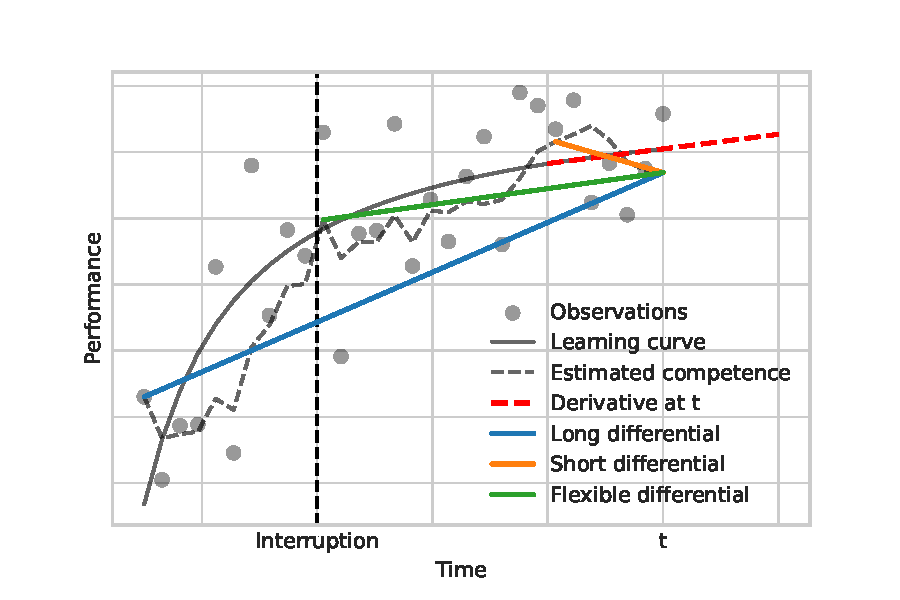
\includegraphics[width=.8\linewidth]{Figures/c5/lptw.pdf}}
    \caption[short figure description]{\textbf{Temporal extent of \ac{LP} estimation}. The plot depicts a hypothetical learning curve on which performance increases with diminishing returns over time. The derivative of this curve represents the true rate of improvement. The learner does not know neither the true learning curve nor its derivative. However, learners compare the estimated performance values at different points in time. Here, the dashed curve represents the box-car estimated learning curve derived from noisy observations (black dots). Note that learning is interrupted for an unspecified period of time (dashed vertical line). Comparing current performance with a very distant reference point is likely to overestimate the derivative (blue line). Comparing it to reference points that are too close in time is unreliable, given the noise in observations (orange line). Resetting the reference point to the beginning of the current episode is more likely to be accurate, if enough attempts are made during the episode (green line).}\label{fig:5-lptw}
\end{figure}

%This situation is similar to the bias-variance tradeoff in statistics and \ac{ML}. While humans might prefer high-bias and low-variance estimates when it come to predicting uncertain quantities \cite{gigerenzer_heuristics_2011}, a more precise specification would be useful.

% Flexible referencing
Fixed time-window computation might be too restrictive to account for the diversity of learning trajectories across different tasks. Shorter time windows are more useful for easier tasks where learning progresses rapidly, while longer time windows are more appropriate for more slowly developing skills. Fixed time-window computation also requires ad hoc assumptions to handle situations in which the reference point extends beyond what is available. For example, given a time window of size $\tau$, the learner would require at least $\tau$ performance evaluations to compute \ac{LP}, unless the parameter is allowed to vary in the beginning. A more flexible approach would be to reset the reference point to when the task is switched to. Such an approach raises the question of how task-disengagement is decided. It turns the relationship between \ac{LP} and its temporal extent upside down: instead of \ac{LP} depending on the fixed time window, the temporal extent of \ac{LP} judgments would depend on the rate of learning (assuming that low \ac{LP} signals the need to disengage from the current task). This temporally flexible \ac{LP} estimation approach is assumed by the psychological \emph{Region of Proximal Learning} theory \parencite{metcalfe_region_2005}, which proposes that once a task is chosen, the amount of time spent on the task will depend on subjective \ac{LP}.

% Summary
In summary, we want to explore the idea that in tasks lacking clear performance feedback (such as precise success rates), \ac{LP} computation is based on performance data that learners decide to monitor. Such data may not correspond to our preconceived objective criteria, so it needs to be validated empirically. What measures learners consider is only one piece of a puzzle. To understand \ac{LP} computation more fully, we also need to understand what they compare the monitored measures to (the question of temporal extent of \ac{LP} estimation). The next section describes an ongoing scientific project aiming to address these questions.